%!TEX root = MemoireZelliges.tex

\chapter{Étude physique d'un zellige noir (\bdx{6530})}
%======================================================================

\section{Description -- État de surface}
%----------------------------------------------------------------------

Cet échantillon, de forme parallélépipédique (\fref{dessin:6530}), est 
une pièce de céramique glaçurée de couleur noire. Il provient du \PaM 
(\siecle{17}) de Meknès.

\begin{itemize}
  \item \DimText : \SI{30x30x21}{\mm}
  \item \emph{Masse} : \SI{20.0}{\g}
\end{itemize}

\begin{figure}[htb]
  \begin{minipage}[b]{3.9cm}
    \centerfloat
    \vspace*{0pt}
    % Dessin de l'échantillon : Vue de dessus
    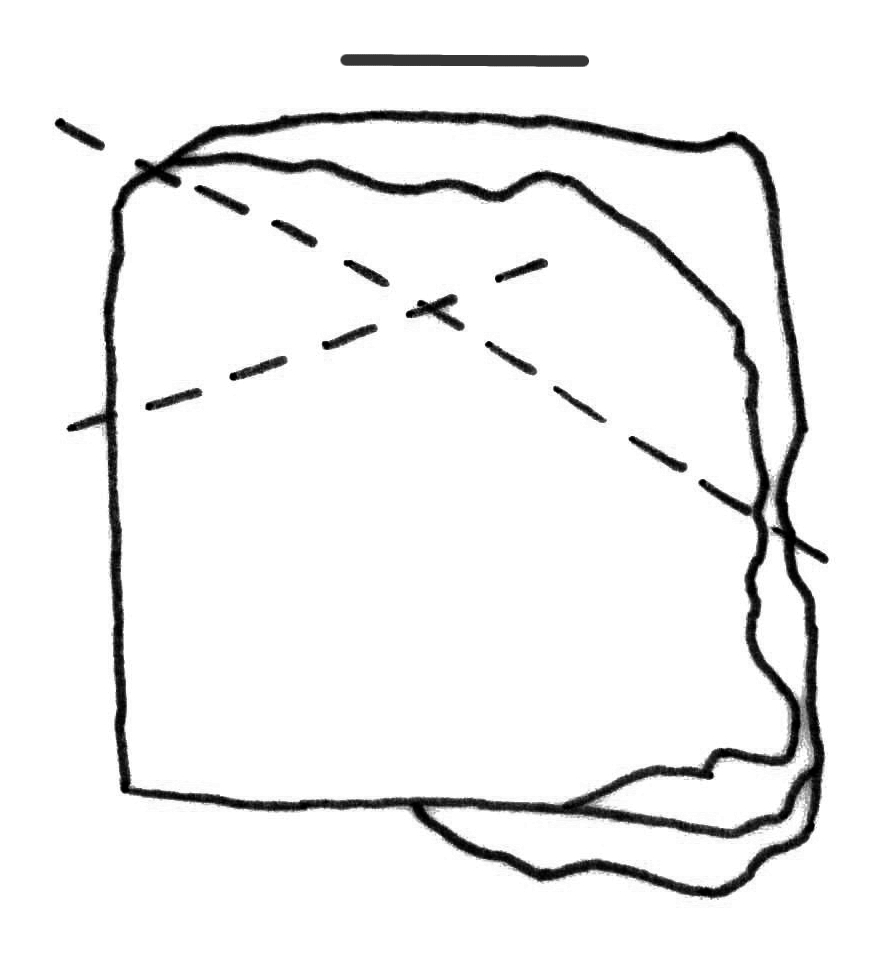
\includegraphics[scale=0.17]{PaM_BDX6530_dessus}
    \subcaption{Vue de dessus \label{dessin:6530_dessus}}

    \bigskip

    % Dessin de l'échantillon : Coupe
    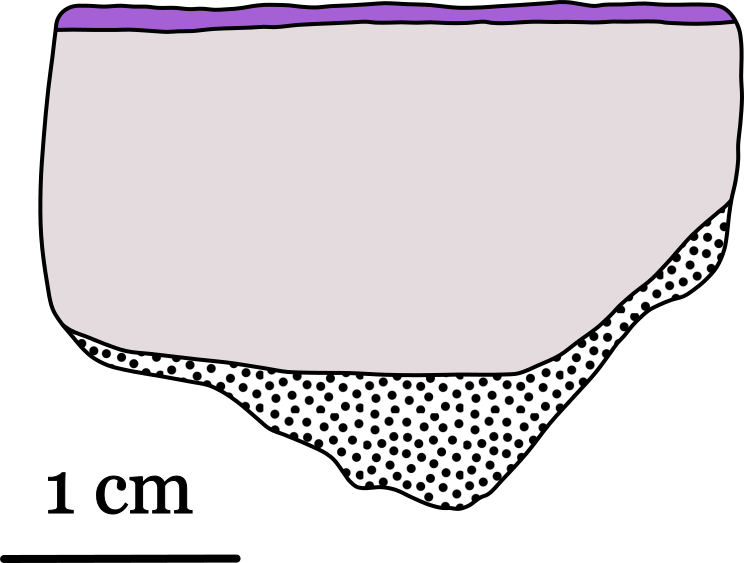
\includegraphics[scale=0.17]{PaM_BDX6530_coupe}
    \subcaption{Vue en coupe \label{dessin:6530_coupe}}
  \end{minipage}%
  \qquad%
  \begin{minipage}[b]{4.8cm}
    \centerfloat
    \vspace*{0pt}
    % Dessin de l'échantillon : Lame
    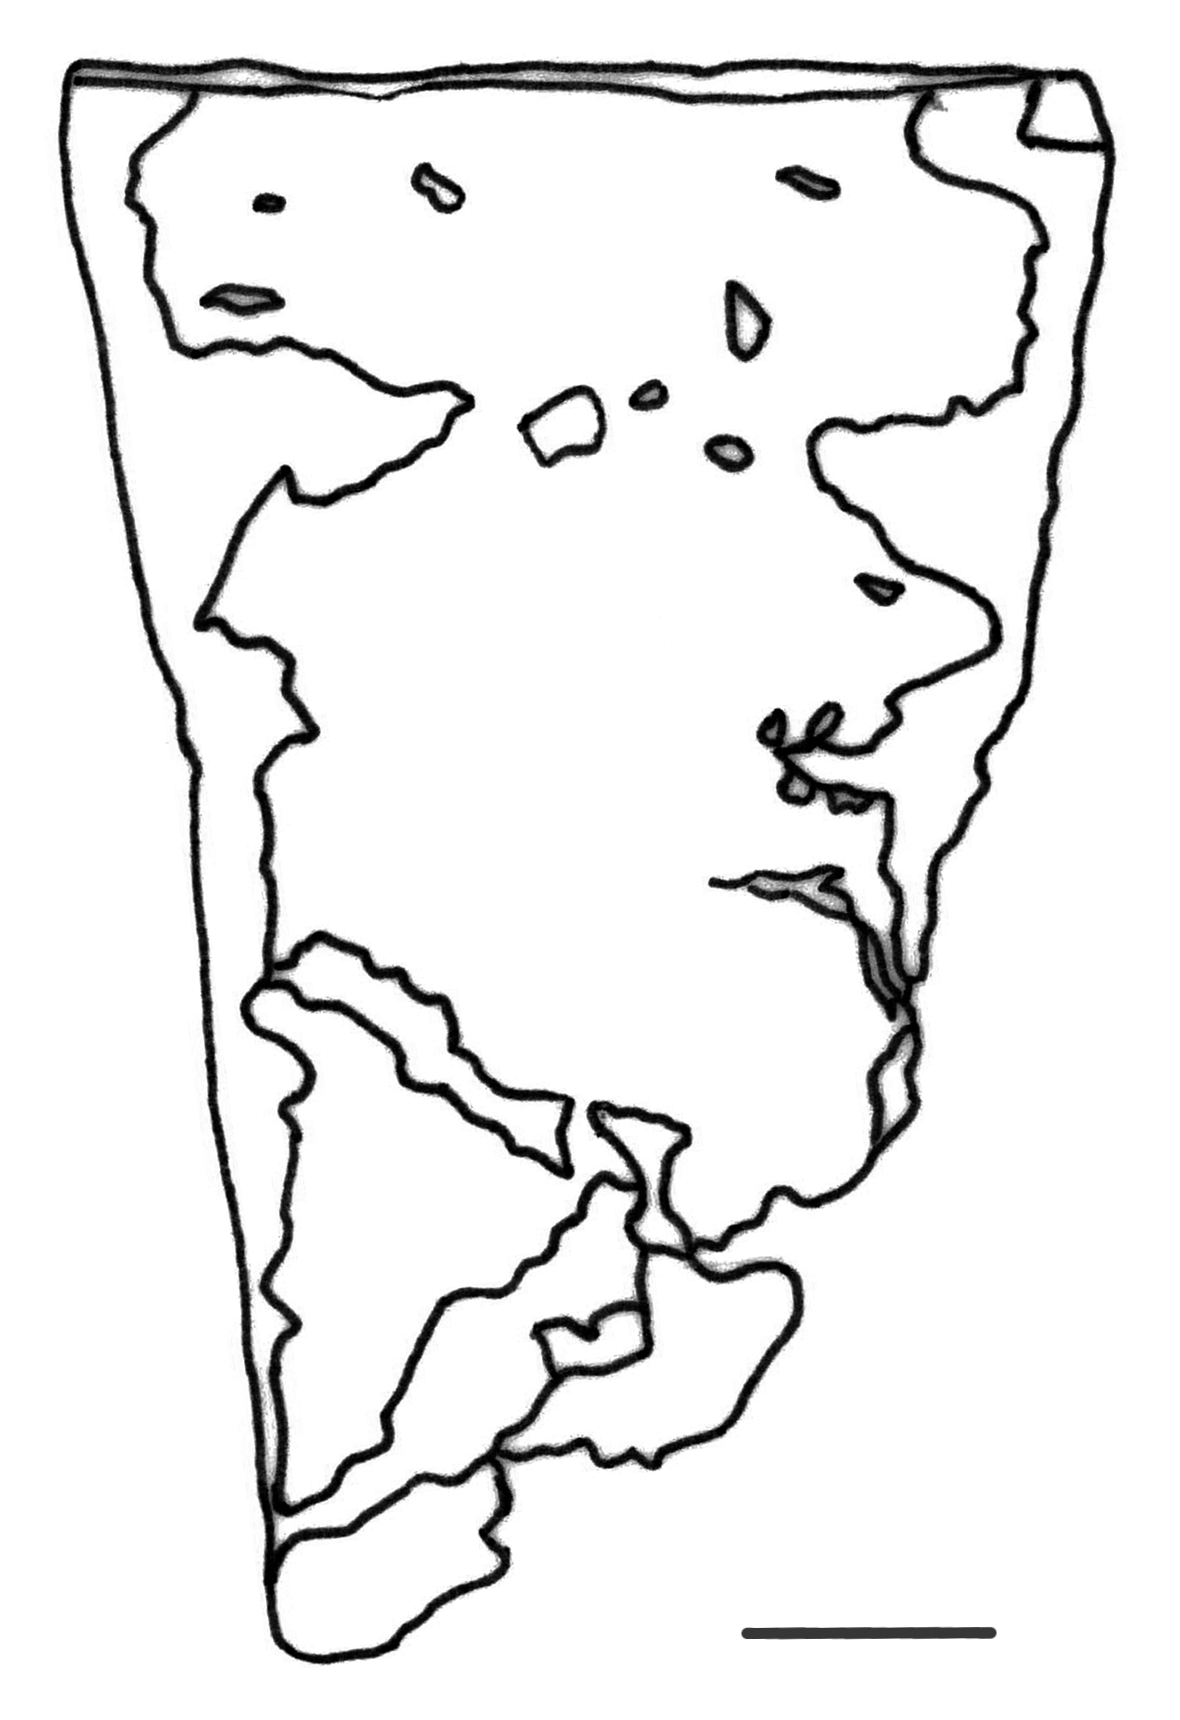
\includegraphics[scale=0.17]{PaM_BDX6530_lame}
    \subcaption{Lame étudiée \label{dessin:6530_lame}}
  \end{minipage}
  \qquad%
  \begin{minipage}[b]{3.2cm}
    \vspace*{0pt}

    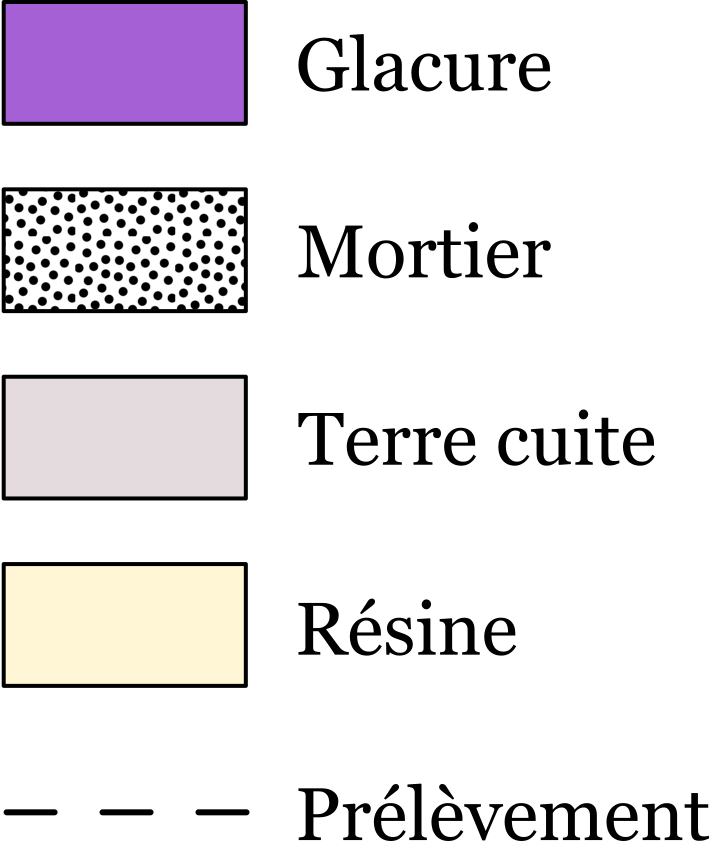
\includegraphics[scale=0.17]{PaM_BDX6530_legende}

    \bigskip
  \end{minipage}
  \caption[\bdx{6530}]{\legendeC.}
  \label{dessin:6530}
\end{figure}

L'observation de la surface de la glaçure (\fref{surf:6530}) montre 
qu'elle contient des bulles, des picots, présente des rayures. On peut 
aussi y remarquer des petits cristaux en forme de baguettes.

Le support de terre cuite est de couleur rosé, de granulométrie fine, 
peu poreux et contient de nombreuses inclusions de tailles et de 
couleurs variées.

\begin{figure}[htb]
  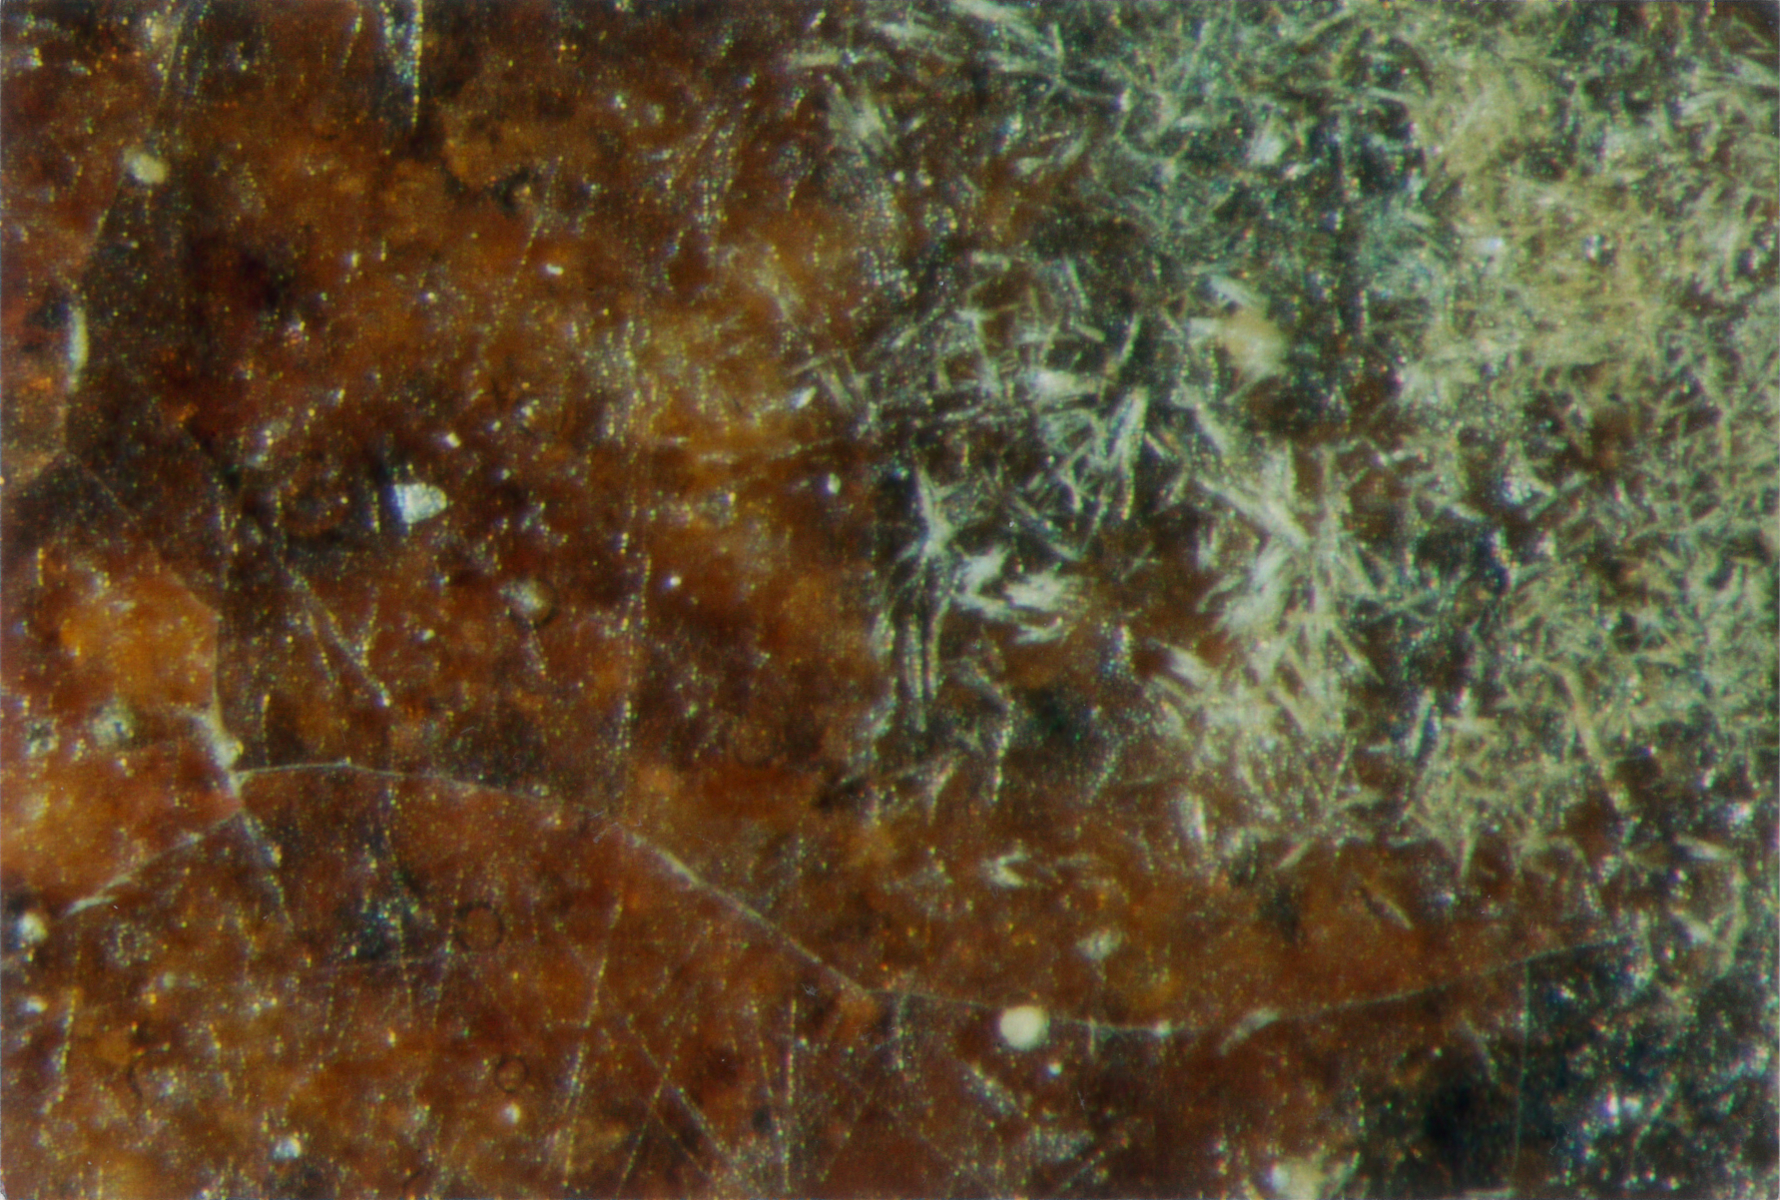
\includegraphics[width=\textwidth]{PaM_BDX6530_Surf}
  \caption[\bdx{6530}\ -- État de surface de la glaçure]
          {\legendeC.
           État de surface de la glaçure 
           (Gr=\num{40}, \zone{\sim3.3x2.4}{\mm}). Elle contient des 
           bulles, des picots et présente des rayures.}
  \label{surf:6530}
\end{figure}


\section{Étude de la couleur}
%----------------------------------------------------------------------

\subsection{Identification des ions chromogènes}
%~~~~~~~~~~~~~~~~~~~~~~~~~~~~~~~~~~~~~~~~~~~~~~~~~~~~~~~~~~~~~~~~~~~~~~
\begin{figure}[htb]
  \begin{plotspectre}
    \addplot [thick, Indigo] 
       table [x=lambda, y=6530gla] {\gladata} ;
    \addplot [thick, FireBrick] 
       table [x=lambda, y=6530tc] {\tcdata} ;
  \end{plotspectre}
  \caption{\legendeC 
           Spectres d'\AO en mode réflexion diffuse de la glaçure et de la terre cuite. Le spectre présente une forte absorption dans tout le domaine visible (\SIrange{400}{700}{\nm}). Il se compose en fait d'une superposition de bandes d'absorption.}
  \label{spectre:6530}
\end{figure}

Le spectre d'\AO en mode réflexion diffuse de la glaçure (\fref{spectre:6530}) présente une forte absorption dans l'ensemble du domaine du visible avec toutefois une transmission un peu plus élevée à partir de \SI{550}{\nm}.

On ne distingue pas de bande d'absorption particulière. Le spectre est 
en fait constitué d'une superposition de bandes d'absorption plus ou 
mois larges et plus ou moins intenses.

La glaçure étant transparente, nous avons également enregistré le 
spectre d'\AO de la terre cuite support. Celui-ci présente une bande 
d'absorption à \SI{440}{\nm} qui correspond au \ch{Fe^3+} 
\autocite{Lajarte_1979}. La bande à \SI{550}{\nm} n'a pu être 
attribuée.

\subsection{Mesure physique de la couleur}
%~~~~~~~~~~~~~~~~~~~~~~~~~~~~~~~~~~~~~~~~~~~~~~~~~~~~~~~~~~~~~~~~~~~~~~
\begin{table}
  \begin{chrotab}
      \chrolgna{Glaçure}{594.39}{8.88}
               {6.505}{0.338}{0.335}
               {30.652}{4.036}{2.934} &
      \chrolgnb{orange très foncé}{Orange}{585}{600}
               {\footcite{Kelly_1976}}
    \tabularnewline
      \chrolgna{Terre cuite}{579.70}{23.30}
               {47.348}{0.359}{0.366}
               {74.412}{3.957}{18.143} &
      \chrolgnb{jaune orange clair}{Jaune-Orange}{580}{585}
               {\footcite{Kelly_1976}}
    \tabularnewline
  \end{chrotab}
  \caption{\legendeC 
           Coordonnées chromatiques dans les systèmes \Yxy et \Lab 
           et longueur d'onde dominante (illuminant D65, \ang{2},
           \SIrange{400}{700}{\nm}).}
  \label{saotab:6530}
  \footnotetext{\autocite{Kelly_1976}}
\end{table}

\begin{figure}[htb]
  \newcommand{\samplename}{6530gla}
  \newcommand{\samplecolor}{Indigo}
  \begin{minipage}[t]{0.37\paperwidth}
    \begin{plotYxy}
      \plotYxyPaV ;
      \plotYxyIlluminant ;
      \plotYxySample{\samplename}{\samplecolor} ;
      \plotYxyLigne{\samplename} ;
      \plotYxyAnnot{\samplename}{south west} ;
    \end{plotYxy}
    \subcaption{espace \trichro \Yxy. La longueur d'onde 
                dominante de la glaçure est de \SI{594.380}{\nm} 
                et correspond au domaine du orange.}
  \end{minipage}%
  \qquad%
  \begin{minipage}[t]{0.37\paperwidth}
    \begin{plotLab}
      \plotLabSample{\samplename}{\samplecolor} ;
    \end{plotLab}
    \subcaption{espace \trichro \Lab.}
  \end{minipage}%
  \caption[\bdx{6530}\ -- Espaces \trichros]
          {\legendeC Analyse chromamétrique de la glaçure.}
  \label{colorfig:6530}
\end{figure}

Les spectres d'\AO de la glaçure et de la terre cuite ont permis de calculer les coordonnées chromatiques correspondant aux espaces \Yxy et \Lab. La longueur d'onde dominante de la glaçure est de \SI{594.39}{\nm} (\tref{saotab:6530}), elle appartient au domaine des orange. La pureté d'excitation indique une couleur très peu saturée et la réflectance $Y$ est celle d'une couleur très foncée. Ce que l'on prend au premier abord pour un noir est en fait un orange très foncé, un noir. La longueur d'onde dominante de la terre cuite (\SI{579.70}{\nm}) se place dans le domaine du jaune-orange. Sa réflectance est assez élevée, la couleur est donc assez claire. La \fref{colorfig:6530} montre la localisation des cordonnées chromatiques de la glaçure noire dans les espaces \Yxy et \Lab.


\section{Étude de la texture de la glaçure et de la terre cuite}
%----------------------------------------------------------------------

\subsection{Observation en lumière naturelle}
%~~~~~~~~~~~~~~~~~~~~~~~~~~~~~~~~~~~~~~~~~~~~~~~~~~~~~~~~~~~~~~~~~~~~~~
\begin{figure}[htb]
  \begin{minipage}[t]{0.4\textwidth}
    \fakeimg{lum. nat.}
    \subcaption{Lumière naturelle \label{texture:6530_LN}}
  \end{minipage}
  \begin{minipage}[t]{0.4\textwidth}
    \fakeimg{Cathodo}
    \subcaption{\CL \label{texture:6530_CL}}
  \end{minipage}
  \caption[\bdx{6530}\ -- Observation de la texture en section]
          {\legendeC 
           Observation de la texture en section sur une surface de 
           \SI{2.6x1.9}{\mm}.}
  \label{texture:6530}
\end{figure}

L'examen en section en lumière naturelle de l'ensemble terre 
cuite/glaçure (\fref{texture:6530_LN}), montre que la glaçure est 
colorée dans la masse et qu'elle adhère bien au support de terre cuite.

Cette dernière contient diverses inclusions de faibles dimensions,
noires, rouges, blanches.

\subsection{Observation en \CL}
%~~~~~~~~~~~~~~~~~~~~~~~~~~~~~~~~~~~~~~~~~~~~~~~~~~~~~~~~~~~~~~~~~~~~~~
La glaçure n'est pas luminescente (\fref{texture:6530_CL}).

La terre cuite présente une luminescence mauve sur laquelle se 
détachent des luminescences ponctuelles rouges et bleues.

On n'observe aucune luminescence à l'interface glaçure/terre cuite.

Les quelques points jaunes que l'on peut remarquer dans la terre cuite 
et à la surface de la glaçure sont des résidus de la suspension 
diamantée utilisée pour le polissage de la lame.

\subsection{Observation en \MEB[ie]}
%~~~~~~~~~~~~~~~~~~~~~~~~~~~~~~~~~~~~~~~~~~~~~~~~~~~~~~~~~~~~~~~~~~~~~~
La glaçure a une épaisseur moyenne de \SI{170}{\um} et contient 
des bulles (\fref{MEB:6530_img}). On distingue des cristaux de 
forme aciculaire dans sa masse et d'autres cristaux à l'interface 
glaçure/terre cuite.

\begin{figure}[htb]
  \fakeimg{Texture au MEB, retrodiff (fig 44)}
  \caption[\bdx{6530}\ -- Observation de la texture au \MEB, 
           en mode \ERD. Ensemble glaçure/terre cuite]
          {\legendeC
           Observation de la texture au \MEB, en mode \ERD. 
           Ensemble glaçure/terre cuite. La barre d'échelle mesure 
           \SI{200}{\um} (\zone{550x440}{\um}).}
  \label{MEB:6530_img}
\end{figure}

Une \carto de \RX de l'ensemble terre cuite/glaçure (\fref{MEB:6530_carto_tcgla}) met en évidence la présence de manganèse et de plomb dans la glaçure. Elle est en revanche plus pauvre en calcium, aluminium et potassium que la terre cuite. Les cristaux de forme aciculaires se développant dans la masse de la glaçure semblent riches en calcium et manganèse mais dépourvus de plomb.

\begin{figure}[htb]
  \fakeimg{Texture au MEB, carto tc/gla (fig 45)}
  \caption[\bdx{6530}\ -- Observation de la texture au \MEB, \carto de \RX de l'ensemble glaçure/terre cuite]
          {\legendeC
           Observation de la texture au \MEB, \carto de \RX de l'ensemble glaçure/terre cuite (Gr=200, \zone{550x440}{\um}).}
  \label{MEB:6530_carto_tcgla}
\end{figure}

L'interface terre cuite/glaçure présente une forte concentration en 
potassium. Son faible développement semble indiquer des interactions 
faibles entre ces deux matériaux et l'on peut donc envisager 
l'hypothèse de l'application du mélange glaçurant sur une terre crue.

La terre cuite contient des inclusions identifiées par \carto de \RX (\fref{MEB:6530_carto_tc}) comme des quartz et des aluminosilicates potassiques.

\begin{figure}[htb]
  \fakeimg{Texture au MEB, carto tc (fig 46)}
  \caption[\bdx{6530}\ -- Observation de la texture au \MEB, \carto de \RX de la terre cuite]
          {\legendeC
           Observation de la texture au \MEB, \carto de \RX de la terre cuite (Gr=150, \zone{730x600}{\um}). La terre cuite contient des inclusions de quartz et d'aluminosilicates potassiques.}
  \label{MEB:6530_carto_tc}
\end{figure}


\section{Composition élémentaire de la glaçure}
%----------------------------------------------------------------------

\begin{table}
  \begin{cartotab}
      \cartolgn{SiO2}{46.37}{0.83} &
      \cartolgn{CaO}{5.92}{0.36}   &
      \cartolgn{Al2O3}{3.97}{0.93} &
      \cartolgn{MgO}{0.99}{0.14}
    \tabularnewline
      \cartolgn{Na2O}{0.40}{0.07}  &
      \cartolgn{K2O}{3.17}{0.61}   &
      \cartolgn{Fe2O3}{2.09}{0.10} &
      \cartolgn{PbO}{32.27}{0.67}
    \tabularnewline
      \cartolgnnd{SnO2} &
      \cartolgnnd{CuO}  &
      \cartolgnnd{CoO}  &
      \cartolgn{MnO}{4.29}{0.34}
    \tabularnewline
      \cartolgnnd{Cr2O3} &
      \cartolgnnd{ZnO}   &
      \cartolgnnd{Sb2O3} &
      \cartolgn{TiO2}{0.24}{0.04}
    \tabularnewline 
      \cartolgn{S}{0.14}{0.06}  &
      \cartolgnnd{P2O5}         &
      \cartolgn{Cl}{0.14}{0.04} &
      \cartolgnnd{As2O3}
    \tabularnewline
  \end{cartotab}
  \caption[\bdx{6530}\ -- Analyse quantitative par \EDS, composition élémentaire de la 
           glaçure]
          {\legendeC Analyse quantitative par \EDS. Composition élémentaire de la glaçure 
           noire sur une surface de \SI{108x88}{\um} (\PMO).}
  \label{compelem:6530_gla}
\end{table}

La glaçure est plombifère (\SI{32.27}{\percent} de \ch{PbO}) et non 
opacifiée. Elle est colorée par le \ch{Mn^3+} (\SI{4.29}{\percent} 
de \ch{MnO}) en cuisson oxydante. Cet élément, qui présente une 
absorption vers \SI{500}{\nm}, donne en général une couleur variant 
du rose au violacé. Cependant, la glaçure contient également du fer 
(\SI{2.09}{\percent} de \ch{Fe2O3}), sous la forme \ch{Fe^3+}. C'est 
ce dernier, dont les bandes d'absorption se situent dans le bleu 
(\SIlist{380;440}{\nm}), qui modifie la couleur pour donner un orange 
très foncé \autocite{Lajarte_1979}.


\section{Étude de la terre cuite support}
%----------------------------------------------------------------------

\subsection{Composition élémentaire}
%~~~~~~~~~~~~~~~~~~~~~~~~~~~~~~~~~~~~~~~~~~~~~~~~~~~~~~~~~~~~~~~~~~~~~~
\begin{table}
  \begin{cartotab}
      \cartolgn{SiO2}{53.57}{1.17}  &
      \cartolgn{CaO}{17.88}{0.58}   &
      \cartolgn{Al2O3}{14.01}{0.40} &
      \cartolgn{MgO}{3.25}{0.05}
    \tabularnewline
      \cartolgn{Na2O}{0.58}{0.03}  &
      \cartolgn{K2O}{1.91}{0.20}   &
      \cartolgn{Fe2O3}{7.20}{0.50} &
      \cartolgnnd{PbO}
    \tabularnewline
      \cartolgnnd{SnO2} &
      \cartolgnnd{CuO}  &
      \cartolgnnd{CoO}  &
      \cartolgnnd{MnO}
    \tabularnewline
      \cartolgnnd{Cr2O3} &
      \cartolgnnd{ZnO} &
      \cartolgnnd{Sb2O3} &
      \cartolgn{TiO2}{0.83}{0.08}
    \tabularnewline 
      \cartolgn{S}{0.27}{0.03}    &
      \cartolgn{P2O5}{0.45}{0.05} &
      \cartolgn{Cl}{0.05}{0.01}   &
      \cartolgnnd{As2O3}
   \tabularnewline
  \end{cartotab}
  \caption[\bdx{6530}\ -- Analyse quantitative par \EDS, composition élémentaire de la 
           glaçure]
          {\legendeC Analyse quantitative par \EDS. Composition élémentaire de la terre 
           cuite sur une surface de \SI{108x88}{\um} (\PMO).}
  \label{compelem:6530_tc}
\end{table}

La terre cuite est riche en calcium (\tref{compelem:6530_tc}). Sa 
coloration ocre rose est due au \ch{Fe^3+} en atmosphère de cuisson 
oxydante \autocite{Echallier_1984}.

\subsection{Composition \cristallo}
%~~~~~~~~~~~~~~~~~~~~~~~~~~~~~~~~~~~~~~~~~~~~~~~~~~~~~~~~~~~~~~~~~~~~~~
\begin{figure}[htb]
  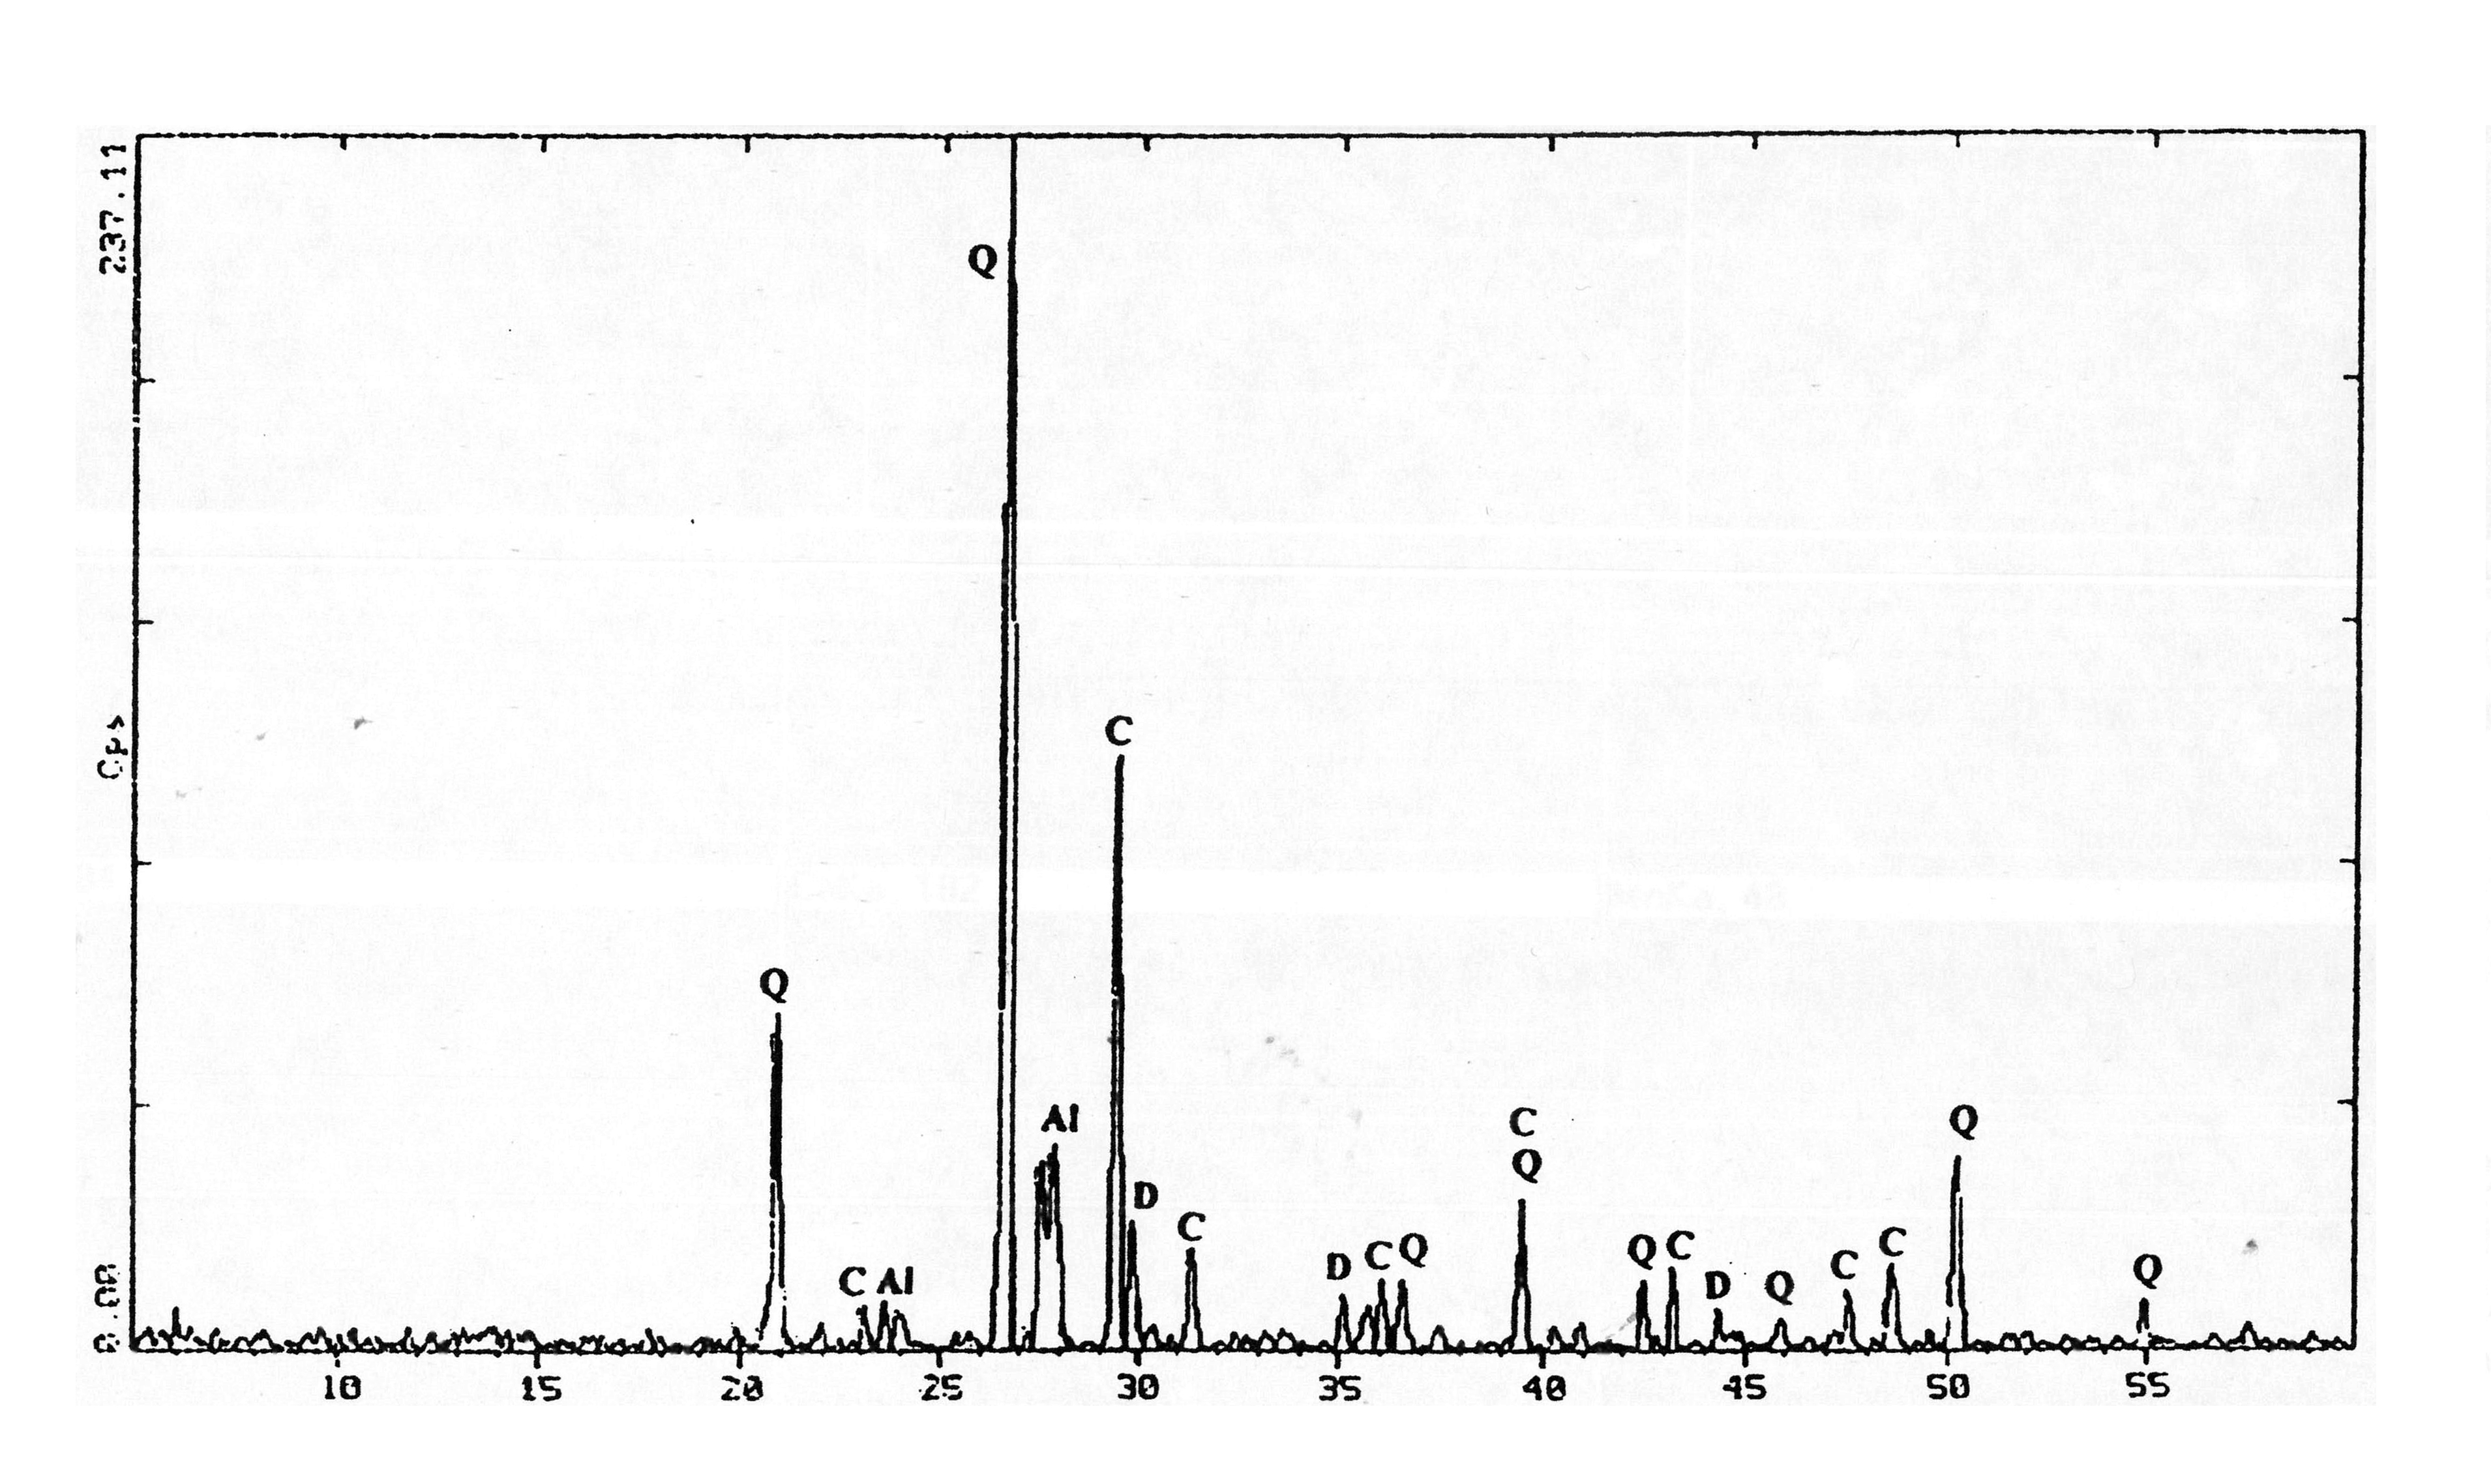
\includegraphics[width=\textwidth]{PaM_BDX6530_DX}
  \caption[\bdx{6530}\ -- \DX sur poudre de la terre cuite]
          {\legendeC 
           \DX sur poudre de la terre cuite. 
           Mise en évidence de la présence de quartz (Q), calcite (C), 
           albite (Al), diopside (D).}
  \label{DRX:6530}
\end{figure}

Le principal composé cristallisé mis en évidence par \DX sur poudre 
(\fref{DRX:6530}) est le quartz (\quartz). La terre cuite contient 
également de la calcite (\calcite), responsable des luminescences 
rouges détectées en \CL. L'albite (\albite) et le diopside (\diopside) 
sont également détectés.

La présence simultanée d'albite et du diopside, une phase haute 
température, laisse supposer que la température maximale de cuisson 
de la céramique a été de l'ordre de \SIrange{850}{900}{\degC}.


\section{Sur la présence et l'identification de cristaux de 
         dévitrification}
%----------------------------------------------------------------------

\subsection{Cristaux se développant dans la masse de la glaçure}
%~~~~~~~~~~~~~~~~~~~~~~~~~~~~~~~~~~~~~~~~~~~~~~~~~~~~~~~~~~~~~~~~~~~~~~
Ces cristaux aciculaires (\fref{MEB:6530_img_cxgla}) ont été 
identifiés par cartogarphie de \RX (\fref{MEB:6530_carto_cxgla}) et 
par des analyses ponctuelles (\tref{compelem:6530_cxgla}).

\begin{table}
  \begin{cartotab}
      \cartolgn{SiO2}{51.64}{0.75} &
      \cartolgn{CaO}{21.25}{2.08}  &
      \cartolgn{Al2O3}{1.95}{0.46} &
      \cartolgn{MgO}{2.83}{0.36}
    \tabularnewline
      \cartolgn{Na2O}{0.19}{0.07} &
      \cartolgn{K2O}{1.30}{0.32}  &
      \cartolgnnd{Fe2O3}          &
      \cartolgn{PbO}{7.97}{1.01}
    \tabularnewline
      \cartolgnnd{SnO2} &
      \cartolgnnd{CuO}  &
      \cartolgnnd{CoO}  &
      \cartolgn{MnO}{12.50}{0.64}
    \tabularnewline
      \cartolgnnd{Cr2O3} &
      \cartolgnnd{ZnO}   &
      \cartolgnnd{Sb2O3} &
      \cartolgnnd{TiO2}
    \tabularnewline
      \cartolgn{S}{0.23}{0.05} &
      \cartolgnnd{P2O5}        &
      \cartolgnnd{Cl}          &
      \cartolgnnd{As2O3}
    \tabularnewline
  \end{cartotab}
  \caption[\bdx{6530}\ -- Analyse quantitative par \EDS, composition élémentaire des 
           cristaux se développant dans la glaçure]
          {\legendeA Analyse quantitative par \EDS. Composition élémentaire des cristaux 
           se développant dans la glaçure par analyses ponctuelles 
           (\SI{1}{\um\squared}) (\PMO).}
  \label{compelem:6530_cxgla}
\end{table}

\begin{figure}[htb]
  \fakeimg{Carto RX cristaux glaçure (fig 48)}
  \caption[\bdx{6530}\ -- \carto de \RX des cristaux se développant dans la glaçure]
          {\legendeC 
           \carto de \RX des cristaux se développant dans la glaçure (Gr=2000, \zone{55x45}{\um}). Ces cristaux sont riches en calcium et manganèse.}
  \label{MEB:6530_carto_cxgla}
\end{figure}

Ce sont des silicates calciques de manganèse et de plomb. Leurs formes 
indiquent qu'il s'agit de cristaux de néoformation.

\begin{figure}[htb]
  \fakeimg{6530ER92 (fig 49)}
  \caption[\bdx{6530}\ -- Image en mode \ERD, cristaux aciculaires 
           se développant dans la masse de la glaçure]
          {\legendeC 
           Image en mode \ERD. Cristaux aciculaires se développant 
           dans la masse de la glaçure. La barre d'échelle mesure 
           \SI{10}{\um} (\zone{135x30}{\um}).}
  \label{MEB:6530_img_cxgla}
\end{figure}

\subsection{Cristaux se développant à l'interface}
%~~~~~~~~~~~~~~~~~~~~~~~~~~~~~~~~~~~~~~~~~~~~~~~~~~~~~~~~~~~~~~~~~~~~~~
Il s'agit de cristaux de dévitrification, de forme aciculaire, qui se 
développent pendant le refroidissement lent de la glaçure à partir de 
germes formés à haute température.

Nous avons réalisé des analyses ponctuelles pour en déterminer la 
composition élémentaire (\tref{compelem:6530_cx}).

\begin{table}
  \begin{cartotab}
      \cartolgn{SiO2}{55.47}{3.96}  &
      \cartolgn{CaO}{8.44}{2.15}    &
      \cartolgn{Al2O3}{16.57}{2.43} &
      \cartolgn{MgO}{2.26}{0.69}
    \tabularnewline
      \cartolgn{Na2O}{0.86}{0.34}  &
      \cartolgn{K2O}{6.39}{1.60}   &
      \cartolgn{Fe2O3}{5.07}{1.71} &
      \cartolgn{PbO}{3.59}{0.99}
    \tabularnewline
      \cartolgnnd{SnO2} &
      \cartolgnnd{CuO}  &
      \cartolgnnd{CoO}  &
      \cartolgn{MnO}{0.97}{0.23}
    \tabularnewline
      \cartolgnnd{Cr2O3} &
      \cartolgnnd{ZnO}   &
      \cartolgnnd{Sb2O3} &
      \cartolgn{TiO2}{0.39}{0.06}
    \tabularnewline
      \cartolgnnd{S}    &
      \cartolgnnd{P2O5} &
      \cartolgnnd{Cl}   &
      \cartolgnnd{As2O3}
    \tabularnewline
  \end{cartotab}
  \caption[\bdx{6530}\ -- Analyse quantitative par \EDS, composition élémentaire des 
           cristaux de dévitrification]
          {\legendeC Analyse quantitative par \EDS. Composition élémentaire des 
           cristaux de dévitrification par analyses ponctuelles
          (\SI{1}{\um\squared}) (\PMO).}
  \label{compelem:6530_cx}
\end{table}

Ces cristaux sont des aluminosilicates calco-potassiques. Ils 
contiennent également du fer.


\section{Étude des altérations de la glaçure}
%----------------------------------------------------------------------

Aucune figure d'altération n'a été mise en évidence dans la glaçure, 
ni visuellement, ni en \MEB[ie] (MEB).


\section{Bilan}
%----------------------------------------------------------------------

Cet échantillon est donc une pièce de céramique portant une glaçure 
plombifère dont la coloration \frquote{noire} est due au \ch{Mn^3+} 
associé au \ch{Fe^3+} en atmosphère de cuisson oxydante.

Son support de terre cuite est de type calcique. Sa coloration ocre-
rose est due à la présence de \ch{Fe^3+} en atmosphère de cuisson 
oxydante.

Sa composition \cristallo (quartz, calcite, albite, diopside) 
laisse penser qu'elle a été cuite à une température de l'ordre de 
\SIrange[range-phrase=\ à\ ]{850}{900}{\degC}.

À l'interface glaçure-terre cuite, on n'observe pas de luminescence. 
Cependant, cette zone renferme des cristaux de dévitrification 
identifiés comme des des aluminosilicates calco-potassiques contenant 
également du fer. Le faible développement de cette zone laisse 
envisager l'application du mélange glaçurant sur une terre cuite.

On note aussi la présence d'un autre type de cristaux de 
dévitrification dans la masse de la glaçure : des silicates calciques 
de manganèse et de plomb.

La glaçure ne présente pas de figure d'altération d'origine chimique 
mais une usure mécanique de surface.
